% MedVision manuscript -- Methods section
% Citation keys are defined in methodology_references.bib.

\section{Methods}\label{sec:methods}

\subsection{Study design and analysis scope}\label{sec:study-design}
We conducted a controlled audit of a medical vision--language classifier. The
estimand was the incremental image contribution when the report remained
available. The principal intervention replaced each radiograph with a uniform
gray tensor while retaining the text, label, architecture, and evaluation
protocol. Full multimodal predictions were compared with this control and with
text-only and image-only models.

The replication unit for confirmatory inference was a trained model at a fixed
seed. Eight seeds (42, 123, 456, 789, 1010, 1111, 1212, 1313) were used for
baseline CADQ, the LearnedMixinFusion text-prior variant (LMH),
Noise-Consistency, and Adaptive-CADQ. The exploratory grounding-aware variant
(GACR-B) was added after the initial plan. Because the same test studies recur
across seeds, subjects were not treated as independent observations across
seeds. ICM was the primary diagnostic; calibration and gate behaviour were
secondary outcomes. The Adaptive-CADQ extension and GACR-B are labelled
post hoc.

Figure~\ref{fig:cohort-flow} records the complete cohort-construction path and
the patient-level analysis split. Figure~\ref{fig:method-workflow} summarizes
the corresponding audit workflow from data provenance through paired inference.

\begin{figure}[pos=htbp]
\centering
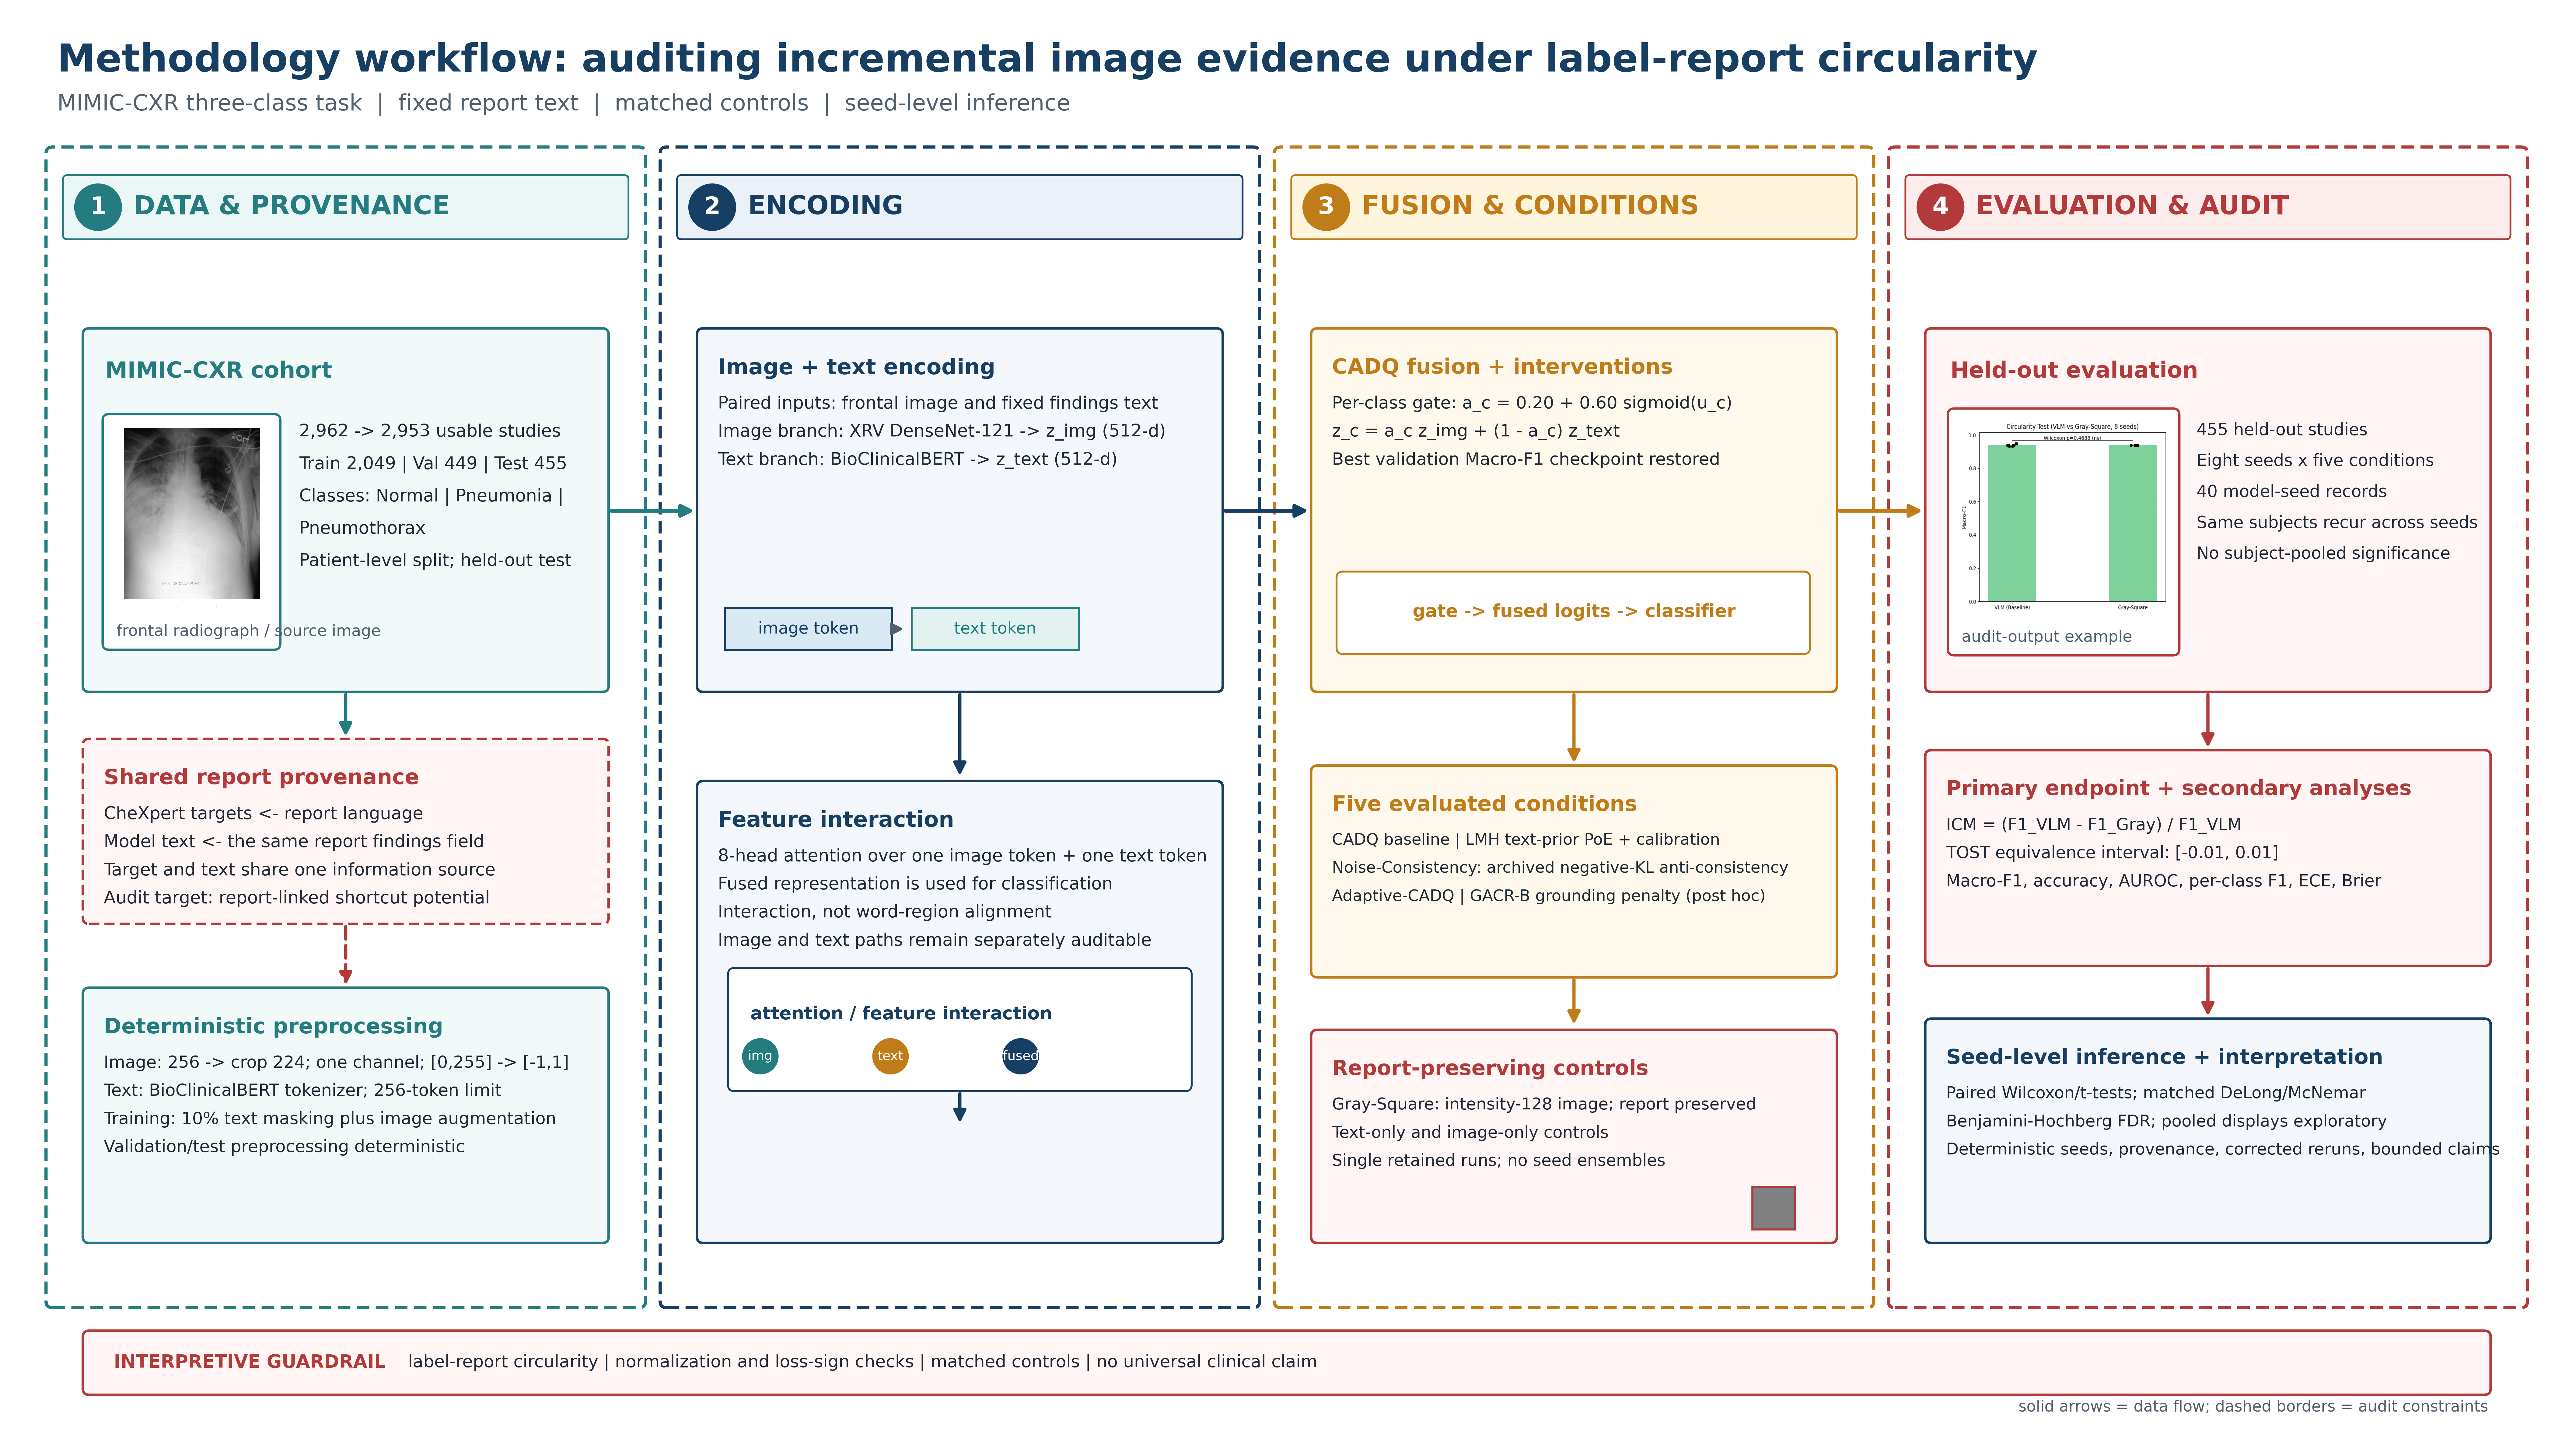
\includegraphics[width=\linewidth]{figures/methodology_audit_workflow_visual_v2.png}
\caption{Audit workflow from MIMIC-CXR data provenance and patient-level splitting
through image/text encoding, CADQ fusion, report-preserving controls, and
seed-level paired inference.}
\label{fig:method-workflow}
\end{figure}

\begin{figure}[pos=htbp]
\centering
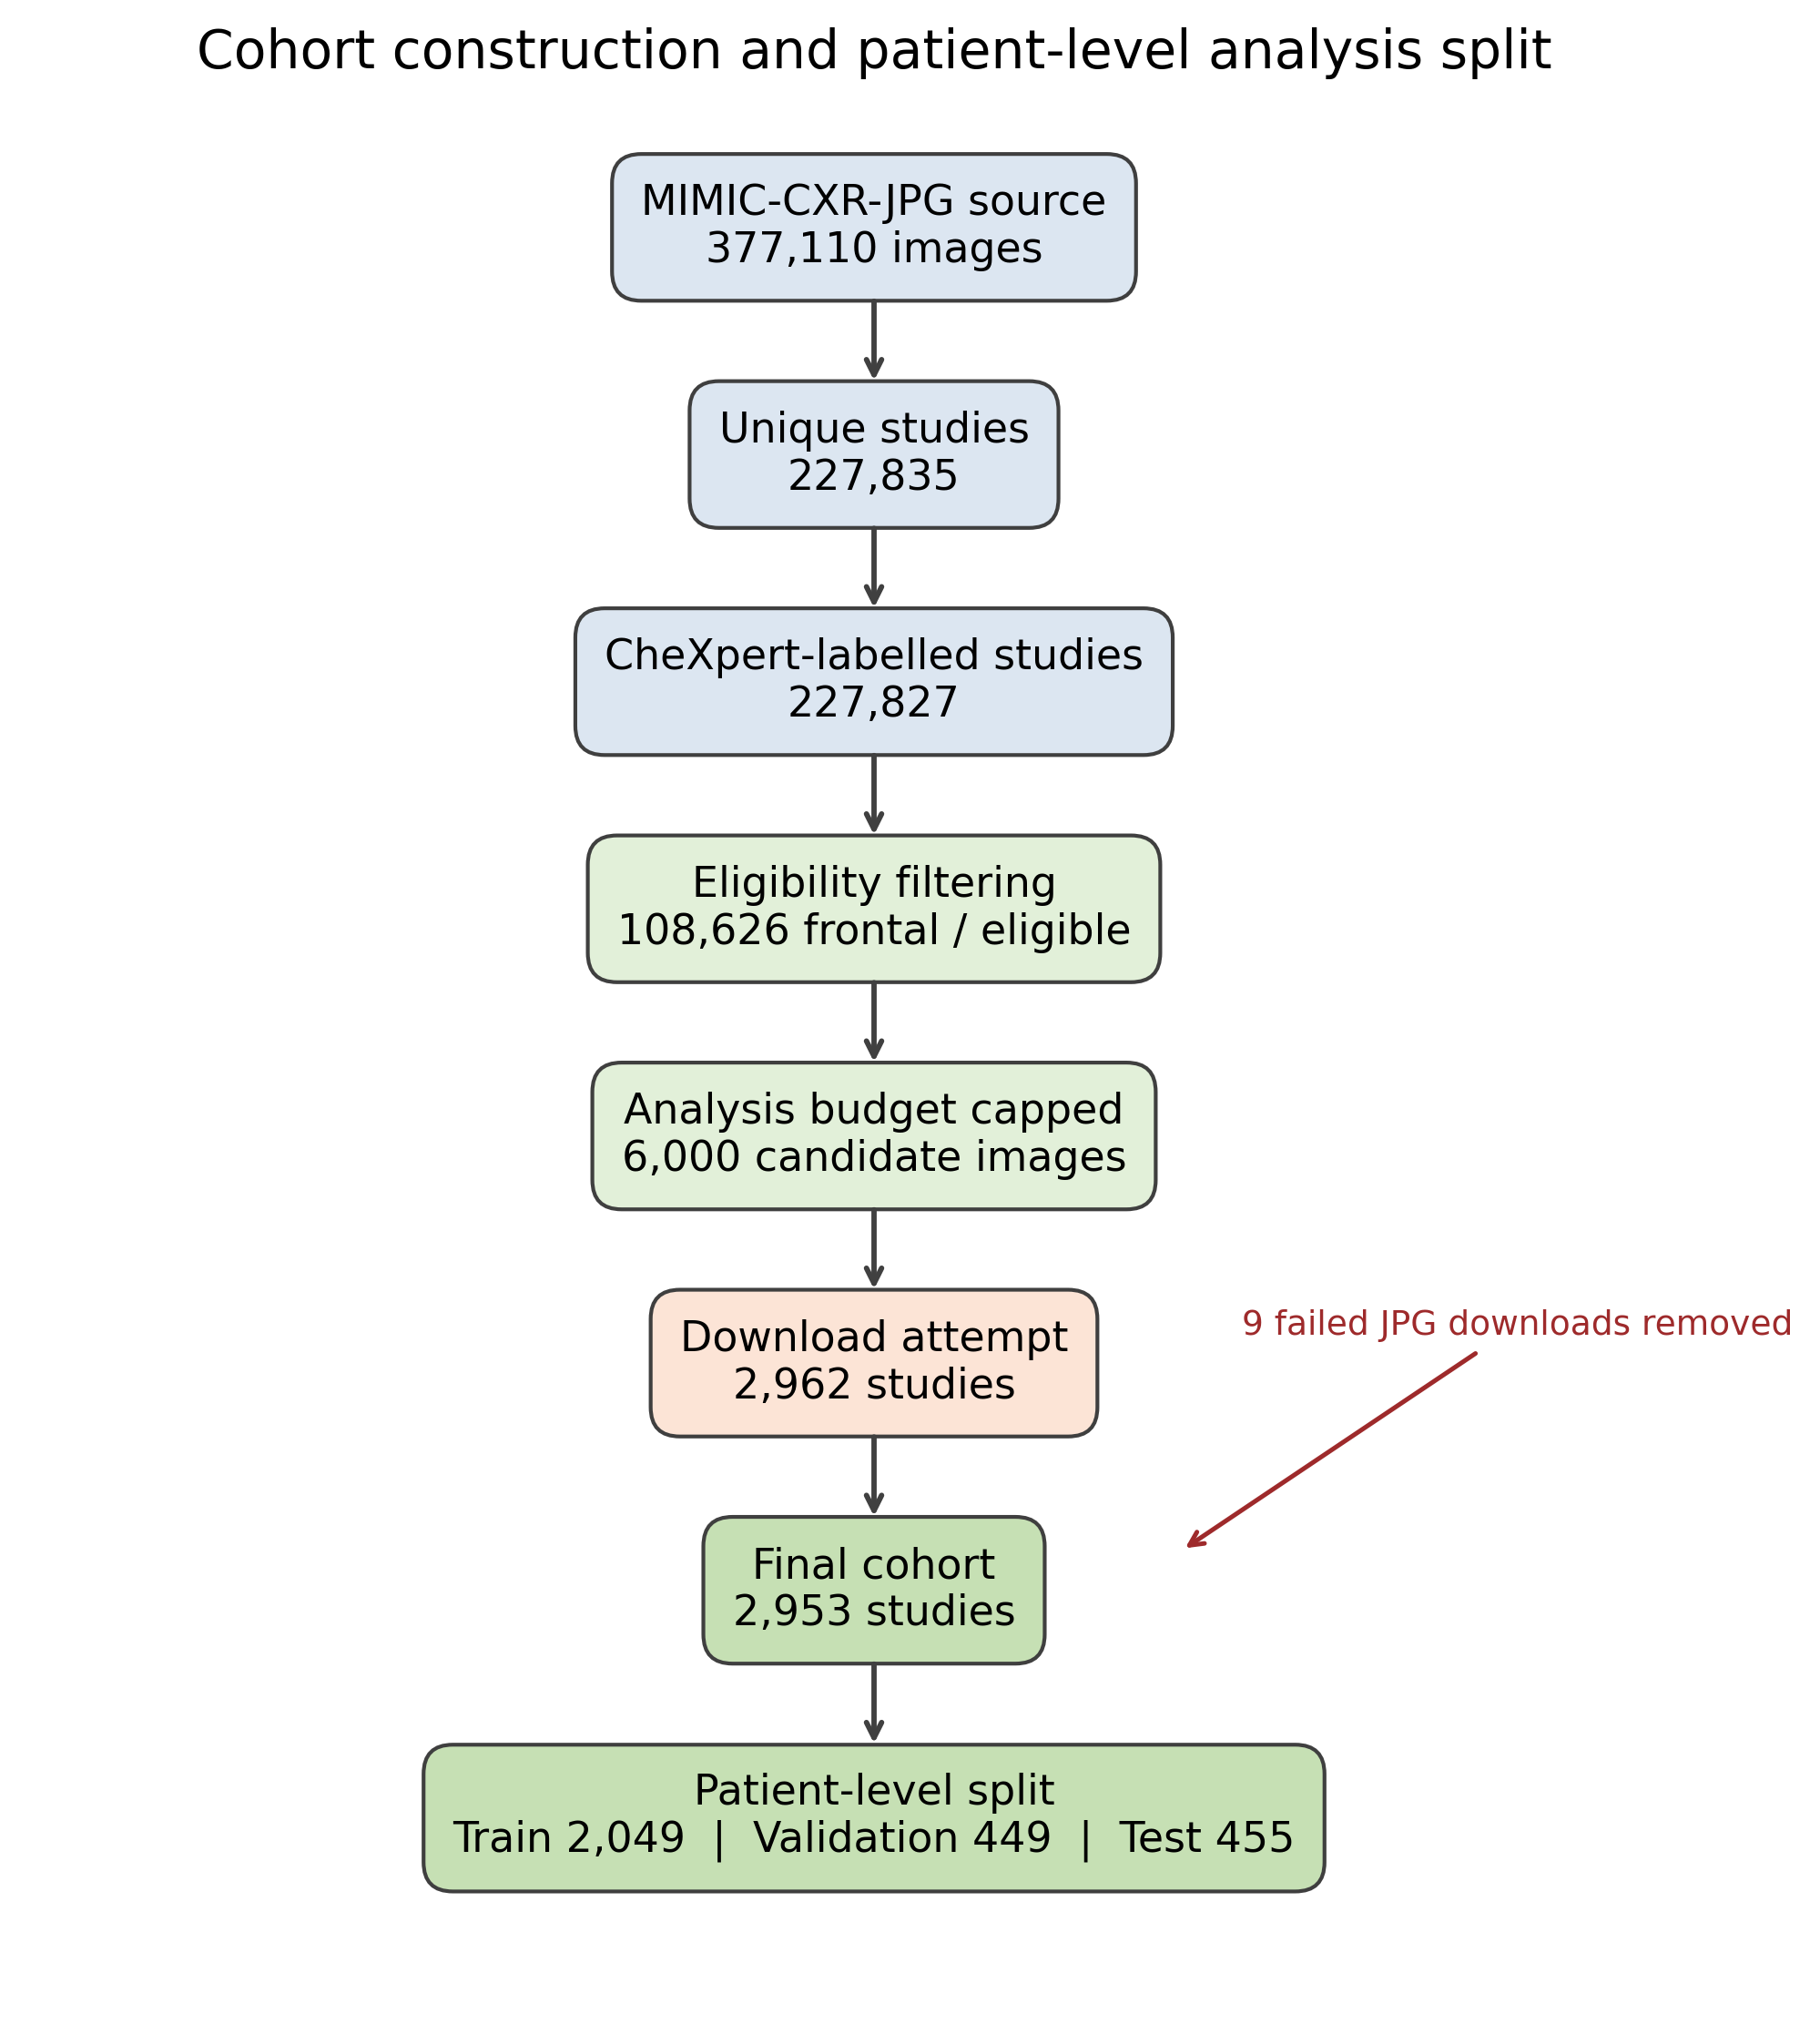
\includegraphics[width=0.52\linewidth]{figures/cohort_flow.png}
\caption{Cohort construction and patient-level analysis split. Nine failed JPG
downloads were removed before the final 2,953-study cohort was partitioned.}
\label{fig:cohort-flow}
\end{figure}

\subsection{Data source and cohort construction}\label{sec:data-cohort}
MIMIC-CXR JPG images and reports were accessed through PhysioNet credentialing
and the applicable Data Use Agreement \citep{johnson2019mimiccxr}. From 2,962
candidate records, nine missing JPG files were removed, leaving 2,953 studies
(2,049 training, 449 validation, and 455 test). Only frontal radiographs were
retained. The three classes were Normal, Pneumonia, and Pneumothorax; class
caps were 2,500, 2,500, and 1,000, respectively. The inherited patient-level
split contained no subject overlap and 47 Pneumothorax studies in the test set.
For transparency, the source-to-analysis flow was 377,110 JPG images, 227,835
unique studies, 227,827 CheXpert-labelled studies, 108,626 eligible frontal
studies, a 6,000-candidate analysis cap, 2,962 download attempts, and 2,953
retained studies after the nine download failures (Fig.~\ref{fig:cohort-flow}).

CheXpert generated the targets from report language using the project’s
uncertain-to-negative mapping \citep{irvin2019chexpert}. The model received the
same report’s \texttt{findings} field. Thus, the experiment audits
label--report circularity rather than an independent image-only diagnostic
task. This secondary analysis used de-identified data; no participants were
recruited and no direct identifiers were accessed. MIMIC-CXR was released for
credentialed research under the source-study IRB approvals; no additional
local participant recruitment or intervention was undertaken for this audit.

\subsection{Preprocessing}\label{sec:preprocessing}
Findings text was tokenized with the
\texttt{emilyalsentzer/Bio\_ClinicalBERT} tokenizer and truncated or padded to
256 tokens. During training, 10\% of strings were replaced by an empty string;
validation and test text was unmasked. Images were resized to $256\times256$,
randomly cropped to $224\times224$, converted to one channel, and mapped from
$[0,255]$ to $[-1,1]$. Training used horizontal flips, rotation (up to
$10^{\circ}$), translation (5\%), and brightness/contrast jitter (0.2); the
class-aware minority transform increased rotation to $15^{\circ}$ and used
translation up to 10\%, scale 0.9--1.1, shear up to $10^{\circ}$, stronger
jitter (0.3), and Gaussian blur. Validation and test images were deterministically
resized and mapped. The archived $[-1,1]$ mapping may not match the native
TorchXRayVision convention and requires a corrected rerun
\citep{cohen2022torchxrayvision}.

\subsection{Model architecture}\label{sec:architecture}
The image branch used TorchXRayVision (XRV) DenseNet-121 with
\texttt{densenet121-res224-mimic\_ch} weights \citep{huang2017densenet,cohen2022torchxrayvision}.
Its output was projected to 512 dimensions with linear, LayerNorm, Gaussian
Error Linear Unit (GELU), and
dropout (0.25); the convolutional stem and first dense block were frozen. The
text branch used Bio\_ClinicalBERT, with its first four layers frozen, and an
analogous 512-dimensional projection \citep{devlin2019bert,alsentzer2019clinicalbert}.
The projected image was one query token and projected text one key/value token
in an eight-head batch-first attention block with residual LayerNorm. This is a
feature interaction, not token-level word--region alignment; its single-key
attention is degenerate and is not interpreted as causal grounding.

\subsection{Fusion variants and controls}\label{sec:variants}
CADQ produced image and text logits and combined them with a learnable
per-class gate \citep{arevalo2017gmu}:
\begin{equation}
\alpha_c=0.20+0.60\operatorname{sigmoid}(u_c),\qquad
z_c=\alpha_cz^{\mathrm{img}}_c+(1-\alpha_c)z^{\mathrm{text}}_c,
\end{equation}
with $u_c=(-0.5,0,0.5)$ and initial gates approximately
$(0.4265,0.5000,0.5735)$. LMH added a five-fold out-of-fold
term-frequency/inverse-document-frequency (TF--IDF)
logistic text-prior branch (5,000 unigram/bigram features, stop-word removal,
balanced weights), validation temperature calibration, $\epsilon=0.1$
smoothing, an input-dependent prior gate, and an entropy penalty (weight 0.05,
annealed for three epochs) following the product-of-experts debiasing rationale
of Cadene et al. \citep{cadene2019rubi}. It was warm-started from CADQ.

Noise-Consistency added Gaussian image noise ($\sigma=0.25$) and the archived
term $\mathcal{L}_{NC}=-D_{KL}(p_{clean}\|p_{noisy})$ based on
Kullback--Leibler (KL) divergence to a minimised loss. It
therefore rewards divergence and is reported as anti-consistency/noise
sensitivity; a positive-KL rerun is required for a conventional consistency
claim. Adaptive-CADQ replaced the static gate with a sample-dependent scalar
from image/text entropies through a $2\rightarrow16\rightarrow1$ multilayer
perceptron (MLP). GACR-B
used an out-of-fold text baseline and a cosine penalty (weight 0.3) on examples
where that baseline was wrong; it is exploratory and follows the grounding-aware
consistency intervention of Sadanandan and Behzadan
\citep{sadanandan2026consistentdangerous}.

All controls used the same test studies. Image-only used the XRV encoder and a
512-to-256 classifier; text-only used frozen Bio\_ClinicalBERT and a
768-to-256 classifier. Gray-Square replaced each image with a constant
intensity-128 tensor while preserving the report and multimodal path. Retained
image-only and Gray-Square outputs were single runs, not seed ensembles.

\subsection{Training and checkpoint selection}\label{sec:training}
Models were trained for 10 epochs with AdamW \citep{loshchilov2019adamw}, differential learning rates of
$10^{-5}$ for image/text backbones, $10^{-4}$ for fusion and LMH heads, and
$5\times10^{-5}$ for static gates; weight decay was $10^{-4}$. OneCycleLR used
10\% warm-up \citep{smith2019superconvergence}. Physical batch size was 8 with four accumulation steps (effective
32), mixed precision, and gradient scaling. Training used focal
cross-entropy ($\gamma=1.5$), label smoothing 0.05, and effective-number
weights ($\beta=0.99$) \citep{lin2017focalloss}; class-aware sampling replicated
Pneumothorax up to fivefold and Pneumonia up to threefold. The best validation
Macro-F1 checkpoint was restored for multimodal variants. The archived
image-only control did not consistently restore its best state and is
descriptive.

\subsection{Endpoints and statistical analysis}\label{sec:statistics}
The primary endpoint was
\begin{equation}
\mathrm{ICM}=\frac{F1_{VLM}-F1_{Gray}}{F1_{VLM}},
\end{equation}
where positive values indicate an incremental gain from the real image. The two
one-sided tests (TOST) procedure tested equivalence to zero within
$[-0.01,0.01]$, an operational margin rather
than a clinical threshold \citep{lakens2017equivalence}. Per seed, we computed
macro-averaged F1 score (Macro-F1), per-class F1, accuracy, one-versus-rest area under the receiver
operating characteristic curve (Macro-AUROC), confusion matrices, ten-bin
expected calibration error (ECE), and multiclass Brier score. Paired Wilcoxon tests
(Pratt zero handling), paired $t$-tests, bootstrap intervals, and Cohen’s $d$
were used for matched seed differences; ECE/Brier were recomputed from retained
probability arrays and absent outputs were recorded as N/A, never zero.

DeLong AUROC comparisons for correlated curves \citep{delong1988roc} and
McNemar tests for paired classification decisions \citep{mcnemar1947correlated}
were performed within matched seeds; studies were never concatenated across
seeds for confirmatory inference. Any pooled display is exploratory.
Benjamini--Hochberg controlled false-discovery rate within each test family
\citep{benjamini1995fdr}, with two-sided $p<0.05$ nominally. Gate values were
extracted from saved checkpoint logits using the bounded equation above; manual
or hard-coded plot values were excluded.

\subsection{Reproducibility safeguards}\label{sec:reproducibility}
Python, NumPy, and PyTorch seeds were fixed and deterministic cuDNN settings
enabled. Run metadata, validation history, checkpoints, predictions,
probabilities, and configurations were saved. The fixed archive contains
duplicate merge keys without a preserved source-priority rule or hash manifest;
results are therefore tied to this snapshot and require provenance locking.
The normalisation issue, negative-KL implementation, unequal post-hoc history,
and image-only checkpoint discrepancy are reported explicitly. Reporting follows
CLAIM and TRIPOD+AI \citep{mongan2024claim,collins2024tripodai}.
